%----------------------------------------------------------------------------------------
%	PAGE 7
%----------------------------------------------------------------------------------------
\section{Methodology}
\begin{frame}
\sectionpage

\end{frame}


%----------------------------------------------------------------------------------------
%	PAGE 8
%----------------------------------------------------------------------------------------
\begin{frame}
\frametitle{Model setting}

\begin{itemize}

\item[$\blacksquare$] Considering the following linear model,% (unobservable), %the response vector
\begin{equation}
\label{LM}
\by = {\bX}\bbeta + \varepsilon, \qquad \mathbf{\varepsilon} \sim \mathcal{N}(\bzero,\sigma^2\bI)
\end{equation}
where $\by \in \mathbb{R}^{n}$ is a response vector, $\bX=(\bx_{1},\ldots,\bx_{p})\in \mathbb{R}^{n\times p}$ is a design matrix with columns $\bx_{j}$ and $\bbeta=(\beta_{1}, \ldots, \bbeta_{p}) \t $ is a vector of unknown regression coefficients.
%$X\in {{\mathbb{R}}^{n\times p}}$

\vspace{3mm}

\begin{itemize}
      \item[-]  Standardize the design to $\|\bx_{j}\|^{2}_{2}=n$.

      \medskip

      \item[-] The design matrix $\bX$ is assumed to be deterministic.

\end{itemize}

\end{itemize}


\end{frame}


%----------------------------------------------------------------------------------------
%	PAGE 9
%----------------------------------------------------------------------------------------
\begin{frame}
\frametitle{Least squares estimator}
\begin{itemize}

\item[$\blacksquare$] In classical theory of linear models, the least squares estimator of an estimable regression coefficient $\bbeta_{j}$ can be written as  % (unobservable), %the response vector
\begin{equation}
\hat{\bbeta}^{(lse)}_{j} := (\bx^{\bot}_{j})\t \by /(\bx^{\bot}_{j})\t \bx_{j},
\end{equation}
where $\bx^{\bot}_{j}$ is a projection of $\bx_{j}$ to the orthogonal complement of column space of $\bX_{-j}=(\bx_{k},k\neq j)$.

\item[$\blacksquare$] The $\bx^{\perp}_{j}$ is defined by
\begin{itemize}
      \item[-] $(\bx^{\bot}_{j})\t \bx_{k}=\bzero $, for $ \forall k\neq j$.
      \medskip
      %\item[-] $(\bx^{\bot}_{j})\t \bx_{j}=\|\bx^{\bot}_{j}\|^{2}_{2}$.

\vspace{3mm}

\end{itemize}

\end{itemize}


\end{frame}


%----------------------------------------------------------------------------------------
%	PAGE 10
%----------------------------------------------------------------------------------------
\begin{frame}
\frametitle{Problems}
\begin{itemize}

\item[$\blacksquare$] In high dimensional situation $p>n$, $rank(\bX_{-j})=n$ for all $j$. % (unobservable), %the response vector
\begin{itemize}
\item[$\blacktriangleright$] $\bx^{\bot}_{j}=\bzero$.
\item[$\blacktriangleright$] $\hat{\bbeta}^{(lse)}_{j}$ is undefined.
\end{itemize}
\item[$\blacksquare$] We want to preserve the properties of the least squares estimator.
\begin{itemize}
\item[$\blacktriangleright$] The covariance structure of the least squares estimator:
\end{itemize}
\begin{equation}
\cov(\hat{\bbeta}^{(lse)}_{j},\hat{\bbeta}^{(lse)}_{k})=\sigma^{2} \frac{(\bx^{\bot}_{j})\t \bx^{\bot}_{k}}{\|\bx_{j}\|^{2}_{2}\|\bx_{k}\|^{2}_{2}}
\end{equation}
\item[$\blacksquare$] Motivation of LDPE:
\begin{itemize}
      \item[$\blacktriangleright$] Replace $\bx^{\bot}_{j}$ with $\bz_{j}$.
      \medskip
      \item[$\blacktriangleright$] Relaxing the constraint $\bz_{j}\t \bx_{k}=\bzero$ for $k\neq j$.
\vspace{3mm}

\end{itemize}

\end{itemize}


\end{frame}

%----------------------------------------------------------------------------------------
%	PAGE 11
%----------------------------------------------------------------------------------------
\begin{frame}
\frametitle{Bias-corrected linear estimators}
\begin{itemize}

\item[$\blacksquare$] For any $\bz_{j}$ that is not orthogonal to $\bx_{j}$, the corresponding univariate linear regression estimator satisfies
\begin{equation*}
\hat{\bbeta}^{(lin)}_{j}= \frac{\bz^{T}_{j} \by}{\bz^{T}_{j} \bx_{j}}= \beta_j + \frac{\bz_j^T \varepsilon}{\bz_j^T\bx_j}
+ \sum_{k\neq j}\frac{\bz_j^T\bx_k\beta_k}{\bz_j^T\bx_j}.
\end{equation*}
  \begin{itemize}
  \item[$\blacktriangleright$] Here,  $\hat{\bbeta}^{(lin)}_{j}$ has the same covariance structure with $\hat{\bbeta}^{(lse)}_{j}$.
  \end{itemize}
\item[$\blacksquare$] Note that the bias of $\hat{\bbeta}^{(lin)}_{j}$ is linear in $\beta_k$, which is unbounded. It is impossible to have $\bz_{j}\t \bx_{k}=\bzero$ for all $k\neq j \quad (\bz_{j}\neq\bzero)$. 
\end{itemize}
\end{frame}

%----------------------------------------------------------------------------------------
%	PAGE 12
%----------------------------------------------------------------------------------------
\begin{frame}
\frametitle{Low dimensional projection estimator}
\begin{itemize}

\item[$\blacksquare$] Bias correction with a non-linear initial estimator $\hat{\bbeta}^{(init)}$:
\begin{equation}
\label{LDPE}
\hat{\bbeta}_{j}=\hat{\bbeta}^{(lin)}_{j} - \sum_{k \neq j}\frac{\bz_{j}\t \bx_{k} \hat{\bbeta}^{(init)}_{k} }{\bz^{T}_{j} \bx_{j}}
=\frac{\bz^{T}_{j} \by}{\bz^{T}_{j} \bx_{j}} - \sum_{k \neq j}\frac{\bz_{j}\t \bx_{k} \hat{\bbeta}^{(init)}_{k} }{\bz^{T}_{j} \bx_{j}}.
\end{equation}
   \begin{itemize}
   %\item[$\blacktriangleright$] One-step self-bias correction from $\hat{\bbeta}^{(init)}$:
   %\medskip
   \item[$\blacktriangleright$] The estimation error of $\hat{\bbeta}_{j}$:
   \begin{equation}
   \label{bias(5)}
   \hat{\bbeta}_{j}-\bbeta_{j}=\frac{\bz^{T}_{j} \varepsilon}{\bz^{T}_{j} \bx_{j}} + \frac{\sum_{k \neq j} \bz_{j}\t \bx_{k} (\bbeta_{k} - \hat{\bbeta}^{(init)}_{k}) }{\bz^{T}_{j} \bx_{j}} \triangleq \bA + \bB.
   \end{equation}
   \item[$\blacktriangleright$] It can be viewed as a sum of noise term and bias term.
   %\vspace{3mm}
   \end{itemize}

\end{itemize}


\end{frame}


%----------------------------------------------------------------------------------------
%	PAGE 13
%----------------------------------------------------------------------------------------
\begin{frame}
\frametitle{Error analysis of LDPE$(1)$}
\begin{itemize}

\item[$\blacksquare$] The approximation error of the LDPE (Term $\bB$) can be controlled:
\begin{equation}
\Big|\sum_{k\neq j}\bz_j^T\bx_k(\beta_k-\hbeta_k^{(init)})\Big|
\le \Big(\max_{k\neq j}\big|\bz_j^T\bx_k\big|\Big)\|\hbbeta^{(init)}-\bbeta\|_1.
\end{equation}
\item[$\blacksquare$] For $\bz_{j}$, define
\begin{equation}
\label{defetatau}
\eta_j = \max_{k\neq j}\big|\bz_j^T\bx_k\big|/\|\bz_j\|_2,\qquad \tau_j = \|\bz_j\|_2/|\bz_j^T\bx_j|.
\end{equation}
   \begin{itemize}
   \item[$\blacktriangleright$] Bias factor $\eta_{j}$: $\eta_{j} \|\hat{\bbeta}^{(init)}-\bbeta\|_{1}$ controls the approximation error.
   \item[$\blacktriangleright$] Noise factor $\tau_{j}$: $\tau_{j} \sigma$ is the standard deviation of noise term.
   %\vspace{3mm}
   \end{itemize}

\end{itemize}


\end{frame}


%----------------------------------------------------------------------------------------
%	PAGE 14
%----------------------------------------------------------------------------------------
\begin{frame}
\frametitle{Error analysis of LDPE $(2)$}
\begin{itemize}

\item[$\blacksquare$] Since $\bz_{j} \t \varepsilon \sim N(\bzero, \sigma^{2} \|\bz_{j}\|^{2}_{2})$, equation $(5)$ yields
\begin{equation}
\label{interval}
\eta_{j}\|\hat{\bbeta}^{(init)}-\bbeta\|_{1}/\sigma=o(1)\Rightarrow \tau^{-1}_{j}(\hat{\bbeta}_{j}-\bbeta_{j})\approx N(\bzero,\sigma^{2}).
\end{equation}
\item[$\blacksquare$] Confidence intervals can be constructed by condition (\ref{interval}) and a consistent estimator of $\sigma$.
%\item[$\blacksquare$] Pick a $\bz_{j}$ with a small $\eta_{j}$ for the asymptotic normality and a small $\tau_{j}$ for efficiency of estimation.
\item[$\blacksquare$] Need to solve:
  \begin{itemize}
  \item[$\blacktriangleright$] Choose proper $\bz_{j}$.
  \item[$\blacktriangleright$] Choose $\hat{\bbeta}^{(init)}$.
% \item[$\blacktriangleright$] Estimate $\sigma$.
  \end{itemize}

\end{itemize}
\end{frame}

%----------------------------------------------------------------------------------------
%	PAGE 15
%----------------------------------------------------------------------------------------
\begin{frame}
\frametitle{How can we choose $\bz_{j}$ ?}
\begin{itemize}

\item[$\blacksquare$] Choose $\bz_{j}$ as the residual of lasso:
\begin{small}
\begin{equation}
\label{lasso}
\bz_j = \bx_j - \bX_{-j} \hat{\gamma}_j,\
\hat{\gamma}_j = \mathop{\arg\min}_{\bb}\Big\{\frac{\|\bx_j-\bX_{-j}\bb\|_2^2}{2n}+\lambda_j \|\bb\|_1\Big\}.
\end{equation}
\end{small}
\item[$\blacksquare$] Karush-Kuhn-Tucker conditions for equation (\ref{lasso})  \\
                      $\Rightarrow \quad |\bx_k^T\bz_j/n|\le\lambda_{j}$ for all $k \neq j$ \\
                      \medskip
                      $\Rightarrow \quad \eta_j\le n\lambda_j/\|\bz_j\|_2$.

\end{itemize}


\end{frame}


%----------------------------------------------------------------------------------------
%	PAGE 16
%----------------------------------------------------------------------------------------
\begin{frame}
\frametitle{How can we pick initial estimator of $\bbeta$?}
\begin{itemize}
\item[$\blacksquare$] The scaled lasso is a joint convex minimization method
\begin{equation}
\big\{\hat{\bbeta}^{(init)},\sigma\big\} = \mathop{\arg\min}_{\bb,\sigma}
\Big\{\frac{\|\by-\bX\bb\|_2^2}{2\sigma n} + \frac{\sigma}{2}+\lambda_0\|\bb\|_1\Big\}.
\end{equation}
\item[$\blacksquare$] The scaled lasso is biased, an alternative method scaled lasso-LSE can be applied:
\begin{equation}
\{\hat{\bbeta}^{(init)},\sigma\} = \mathop{\arg\min}_{\bb,\sigma}
\big\{\frac{\|\by-\bX\bb\|_2^2}{2\sigma max(n-|\hat{S}^{(scl)}|,1)} + \frac{\sigma}{2}\big\}
\end{equation}
where $\hat{S}^{(scl)}$ is the set of non-zero estimated coefficients produce by scaled lasso.
%$\bb_j=\bzero \quad \forall j \not\in \hat{S}^{(scl)}$
\end{itemize}
\end{frame}


%----------------------------------------------------------------------------------------
%	PAGE 17
%----------------------------------------------------------------------------------------
%\begin{frame}
%\frametitle{Precedure of LDPE}
%\begin{figure}[h]
%  \centering
%  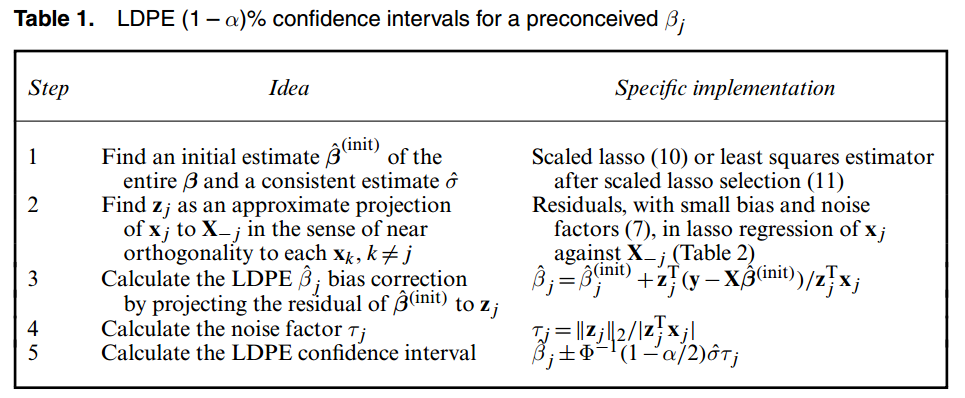
\includegraphics[width=1.0\textwidth]{figs/Table1.png}
%  \label{Table1}
%\end{figure}
%\end{frame}


%----------------------------------------------------------------------------------------
%	PAGE 17
%----------------------------------------------------------------------------------------
\begin{frame}
\begin{block}{Procedure of computing $\bz_{j}$}
    Along the Lasso path for regressing $\bx_j$ against $\bX_{-j}$, let
%Here is a description of the algorithm.
\begin{equation}
\begin{aligned}
\gamma_j(\lambda) = \mathop{\arg\min}_{\bb} \{\|\bx_j & -\bX_{-j}\bb\|_2^2/(2n) + \lambda\|\bb\|_1\}, \\
\bz_j(\lambda)  & = \bx_j-\bX_{-j}\gamma_j(\lambda), \\
\eta_j(\lambda) = \max_{k\neq j} & |\bx_k^T\bz_j(\lambda)|/\|\bz_j(\lambda)\|_2, \\
\tau_j(\lambda)  = & \|\bz_j(\lambda)\|_2/|\bx_j^T\bz_j(\lambda)|, \\
\end{aligned}
\end{equation}
be the coefficient estimator $\gamma_j$, residual $\bz_j$, the bias factor $\eta_j$, and
the noise factor $\tau_j$, as functions of $\lambda$.
\end{block}

\end{frame}


\begin{frame}
  \begin{block}{Proposition 1}
  \scriptsize
  (a) In the Lasso path, $\|\bz_j(\lambda)\|_2$, $\eta_j(\lambda)$, and $\sigma_j(\lambda)$
  are nondecreasing functions of $\lambda$, and $\tau_j(\lambda)\le 1/\|\bz_j(\lambda)\|_2$. Moreover,
  $\gamma_j(\lambda)\neq 0$ implies $\eta_j(\lambda)=\lambda n/\|\bz_j(\lambda)\|_2$. \\
  
  (b) Let $\lambda_{univ}=\sqrt{(2/n)\log p}$. Then,
  \begin{equation}
  \setlength{\abovedisplayskip}{3pt} %%% 3pt 个人觉得稍妥,可自行设置
  \setlength{\belowdisplayskip}{3pt}
  \sigma_j(C\lambda_{univ})>0 \hbox{ iff } \{\lambda>0: \eta_j(\lambda) \le C\sqrt{2\log p}\}\neq \emptyset,
  \end{equation}
      and in this case, the algorithm in Table 2 provides
  \begin{gather}
  \setlength{\abovedisplayskip}{3pt} %%% 3pt 个人觉得稍妥,可自行设置
  \setlength{\belowdisplayskip}{3pt}
  \eta_{j}\leq \eta_j^*\le (1\vee C)\sqrt{2\log p},\\
  \tau_j\le n^{-1/2}(1+\kappa_0)/\hat{\sigma}_j(C\lambda_{univ}).
  \end{gather}
      Moreover, when $\bz_j(0)=\bx_j^\perp =0$, $\eta_j(0+) \inf\{\|\gamma_j\|_1: \bX_{-j}\gamma_j=\bx_j\}=\sqrt{n}$.\\
  (c) Let $0<a_0<1\leq C_0<\infty$. Suppose that for $s=a_0n/\log p$
  \begin{scriptsize}
      \begin{equation*}
      \setlength{\abovedisplayskip}{3pt} %%% 3pt 个人觉得稍妥,可自行设置
      \setlength{\belowdisplayskip}{3pt}
      \inf_{\delta}\sup_{\bbeta}\Big\{\|\delta(\bX,\by) - \bbeta\|_2^2: \by=\bX\bbeta,
      \hbox{$\sum_{j=1}^p$} \min(|\beta_j|/\lambda_{univ},1)\le s+1 \Big\}\le 2C_0s(\log p)/n.
      \end{equation*}
  \end{scriptsize}
  
  \end{block}
\end{frame}

  
%----------------------------------------------------------------------------------------
%	PAGE 19  插入代码表格
%----------------------------------------------------------------------------------------
% \begin{frame}
% \frametitle{Computation of $\bz_{j}$}
% \scriptsize
% \begin{table}%[ht]
% \caption{Computation of $\bz_j$ from the Lasso (\ref{lasso})}
% \begin{tabular}{cl}
% \toprule
% Input: & an upper bound $\eta_j^*$ for the bias factor, with default value $\eta^*_j=\sqrt{2\log p}$, \\
% & tuning parameters $\kappa_0\in [0,1]$ and $\kappa_1\in (0,1]$; \\
% Step 1: & (verify/adjust $\eta_j^*$ and compute the corresponding noise factor $\tau_j^*$) \\
% & If $\eta_j(\lambda)>\eta_j^*$ for all $\lambda>0$, $\eta_j^* \leftarrow (1+\kappa_1)\inf_{\lambda>0}\eta_j(\lambda)$; \\
% & $\lambda\leftarrow \max\{\lambda: \eta_j(\lambda)\le\eta^*_j\}$,
% $\eta_j^*\leftarrow \eta_j(\lambda)$, $\tau_j^*\leftarrow \tau_j(\lambda)$; \\
% Step 2: & (further reduction of the bias factor)\\
% & $\lambda_j \leftarrow \min\{\lambda: \tau_j(\lambda)\le (1+\kappa_0)\tau^*_j\}$;
% \\
% Output: & $\lambda_j$, $\bz_j\leftarrow \bz_j(\lambda_j)$, $\tau_j\leftarrow \tau_j(\lambda_j)$, $\eta_j\leftarrow \eta_j(\lambda_j)$\\
% \bottomrule
% \addlinespace
% \end{tabular}
% \label{table:alg}
% \end{table}
% \end{frame}


%----------------------------------------------------------------------------------------
%	PAGE 18  插入图片 去掉名字
%----------------------------------------------------------------------------------------
\begin{frame}
\frametitle{Computation of $\bz_{j}$}
% \begin{figure}[h]
%   \centering
%   \caption{Computation of $\bz_{j}$ from lasso(12)}
%   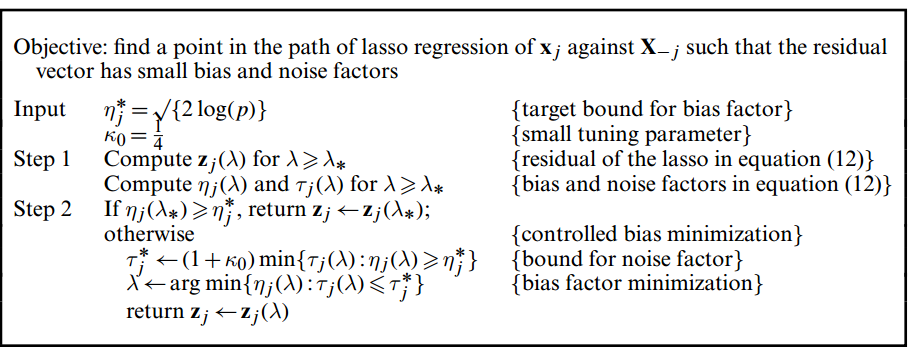
\includegraphics[width=1.0\textwidth]{figs/Table21.png}
%   \label{Table2}
%   \footnote{$lambda_*$ is the smallest non-zero penalty level in the computed lasso path.}
% \end{figure}

% \begin{columns}
  % \begin{column}{0.5\linewidth}
    \begin{table}%[ht]
      \small
      \caption{Computation of $\bz_j$ from the Lasso (12)}
      \begin{tabular}{cl}
      \toprule
      Input: & $\eta^*_j=\sqrt{2\log p}$ \\
      & $\kappa_0 = 0.25$ \\
      Step 1: & Compute $\bz_j$ for $\lambda \geq \lambda_*$, \\
      & Compute $\eta_j$ and $\tau_j$ for $\lambda \geq \lambda_*$ $\eta_j^*$ \\
      Step 2: & If $\eta_j(\lambda_*) \geq \eta_j^*$, return $\bz_j \leftarrow \bz_j(\lambda_*)$; \\
      & otherwise \\
      & $\quad \tau_j^* \leftarrow (1+\kappa_0)\min\{\tau_j(\lambda):\eta_j(\lambda) \geq \eta_j^*\}$ \\ 
      & $\quad \lambda \leftarrow \arg\min \{ \eta_j(\lambda): \tau_j(\lambda)\geq \tau_j^* \}$ \\
      & $\quad \bz_j \leftarrow \bz_j(\lambda)$ \\
      \bottomrule
      \addlinespace
      \end{tabular}
      \footnote{\scriptsize $\lambda_*$ is the smallest non-zero penalty level in lasso path.}
    \end{table}  
  
    % \begin{table}%[ht]
    %   \caption{Computation of $\bz_j$ from the Lasso (ref{Lasso-path-j})}
    %   \begin{tabular}{cl}
    %   \toprule
    %   %\multicolumn{2}{c}{Computation of $\bz_j$ from the Lasso (\ref{Lasso-path-j})}\\ 
    %   % for standardized design vectors}\\ 
    %   %\midrule
    %   Input: & an upper bound $\eta_j^*$ for the bias factor, with default value $\eta^*_j=\sqrt{2\log p}$, \\
    %   & tuning parameters $\kappa_0\in [0,1]$ and $\kappa_1\in (0,1]$; \\
    %   Step 1: & (verify/adjust $\eta_j^*$ and compute the corresponding noise factor $\tau_j^*$) \\
    %   & If $\eta_j(\lambda)>\eta_j^*$ for all $\lambda>0$, $\eta_j^* \leftarrow (1+\kappa_1)\inf_{\lambda>0}\eta_j(\lambda)$; \\
    %   & $\lambda \leftarrow \max\{\lambda: \eta_j(\lambda)\le\eta^*_j\}$, 
    %   $\eta_j^*\leftarrow \eta_j(\lambda)$, $\tau_j^*\leftarrow \tau_j(\lambda)$; \\
    %   Step 2: & (further reduction of the bias factor)\\
    %   & $\lambda_j \leftarrow \min\{\lambda: \tau_j(\lambda)\le (1+\kappa_0)\tau^*_j\}$; 
    %   %%%
    %   \\ 
    %   Output: & $\lambda_j$, $\bz_j\leftarrow \bz_j(\lambda_j)$, $\tau_j\leftarrow \tau_j(\lambda_j)$, $\eta_j\leftarrow \eta_j(\lambda_j)$\\
    %   \bottomrule
    %   \addlinespace
    %   \end{tabular}
    %   % \label{table:alg}
    % \end{table}
%   \end{column}

%   % \begin{column}{0.5\linewidth}
%     \begin{figure}
%       \centering
%       \caption{Computation of $\bz_{j}$ from lasso(12)}
%       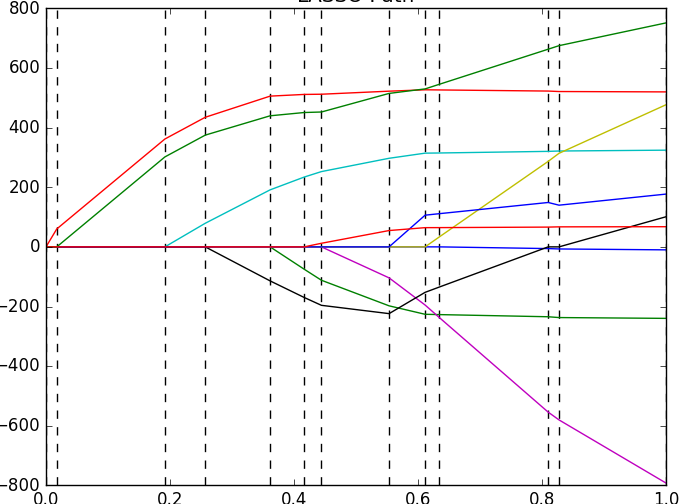
\includegraphics[width=0.5\textwidth]{figs/lasso.png}
%       % \label{Table2}
%     \end{figure}
% %   \end{column}
% \end{columns}
\end{frame}


%----------------------------------------------------------------------------------------
%	PAGE 20
%----------------------------------------------------------------------------------------
%\begin{frame}
%\frametitle{Restricted LDPE}
%\begin{itemize}

%\item[$\blacksquare$] Why use restricted lasso relaxation for $\bz_{j}$?
%  The summands with larger absolute correlation $|\bx_j^T\bx_k/n|$ are likely to have a greater contribution to the bias due to initial estimation error $|\bbeta^{(init)}_k-\beta_k|$.

%\item[$\blacksquare$] How to implement restricted LDPE(RLDPE)?
% Force smaller $|\bz_j^T\bx_k/n|$ for large $|\bx_j^T\bx_k/n|$ with a weighted relaxation:
%\begin{equation}
%\bz_j = \bx_j - \bX_{-j}\gamma_j,\qquad \gamma_j = \argmin_{\bb}{\frac{\|\bx_j-\bX_{-j}\bb\|_2^2}{2n} + \lambda_j\sum_{k\neq j}w_k|b_k|\},
%\end{equation}
%with $w_k$ being a decreasing function of the absolute correlation $|\bx_j^T\bx_k/n|$.
%\item[] Simply set $w_k=0$ for large $|\bx_j^T\bx_k/n|$ and $w_k=1$ for other $k$ in the RLDPE.

%\end{itemize}
%\end{frame}
\begin{frame}
\frametitle{Restricted LDPE}
\begin{itemize}
\item[$\blacksquare$] The reason for using restricted lasso relaxation for $\bz_j$.

  \begin{itemize}
  \item[$\blacktriangleright$]The summands with larger absolute correlation $|\bx_j^T\bx_k/n|$ are likely to have a greater contribution to the bias due to initial estimation error $|\hat{\beta}^{(init)}_k-\beta_k|$.
  \end{itemize}
\item[$\blacksquare$] How to implement restricted LDPE(RLDPE)?
  \begin{itemize}
  \item[$\blacktriangleright$] Force smaller $|\bz_j^T\bx_k/n|$ for large $|\bx_j^T\bx_k/n|$ with a weighted relaxation:
  \end{itemize}
  \begin{scriptsize}
  \begin{equation}
  \bz_j = \bx_j - \bX_{-j}\gamma_j,\quad \gamma_j = \mathop{\arg\min}_{\bb}\left\{\frac{\|\bx_j-\bX_{-j}\bb\|_2^2}{2n} + \lambda_j\sum_{k\neq j}w_k|b_k|\right\},
  \end{equation}
  \end{scriptsize}
%with $w_k$ being a decreasing function of the absolute correlation $|\bx_j^T\bx_k/n|$.

\item[$\blacksquare$] Simply set $w_k=0$ for large $|\bx_j^T\bx_k/n|$ and $w_k=1$ for other $k$ in the RLDPE.

\end{itemize}
\end{frame}


%----------------------------------------------------------------------------------------
%	PAGE 21
%----------------------------------------------------------------------------------------
\begin{frame}
\frametitle{Confidence interval}

\begin{itemize}
\item[$\blacksquare$] The covariance of the noise component in (\ref{bias(5)}) is proportional to
\begin{footnotesize}
\begin{equation}
\bV=(V_{jk})_{p\times p},\quad V_{jk} = \frac{\bz_j^T\bz_k}{|\bz_j^T\bx_j||\bz_k^T\bx_k|}
= \sigma^{-2} cov \Big(\frac{\bz_j^T\varepsilon}{\bz_j^T\bx_j}, \frac{\bz_k^T\varepsilon}{\bz_k^T\bx_k}\Big).
\end{equation}
\end{footnotesize}


\item[$\blacksquare$]
For sparse vectors $\ba$ with bounded $\|\ba\|_0$,
%e.g. $\|\ba\|_0=2$ for a contrast between two regression coefficients,
an approximate $(1-\alpha)100\%$ confidence interval is
\begin{footnotesize}
\begin{equation}
\label{LDPE-CI}
\big|\ba \t \hat{\bbeta} - \ba^T\bbeta\big| \le \hat{\sigma}\Phi^{-1}(1-\alpha/2)(\ba^T\bV\ba)^{1/2},
\end{equation}
\end{footnotesize}
where $\hat{\bbeta} = (\hat{\beta}_1,\ldots,\hat{\beta}_p) \t$ is the vector of LDPEs $\hat{\beta}_j$ in (\ref{LDPE}), $\Phi$ is the standard normal distribution function.

\end{itemize}
\end{frame}

